\documentclass[12pt]{article}

\usepackage[usenames]{color}
\usepackage{listings}
\usepackage{verbatim}
\usepackage{fancyhdr}
\usepackage{graphicx}
\usepackage{amssymb,amsthm}
%\usepackage[fleqn]{amsmath}
\usepackage{amsmath}
% \usepackage[final,notref,notcite,color]{showkeys}
\usepackage[left=1in,top=1in,right=1in,bottom=1in,letterpaper]{geometry}
\renewcommand{\baselinestretch}{1.2}

\pagestyle{fancy}
\lhead{}
\chead{}
\rhead{}
\lfoot{}
\cfoot{\thepage}
\rfoot{}

%
% My edit i added these
%
\allowdisplaybreaks
\usepackage{float}

%% editing
\usepackage[shortlabels]{enumitem}
\usepackage[normalem]{ulem}

%% macros for commenting
\usepackage{mathtools}
\usepackage[normalem]{ulem} % to use \sout

%% math packages
% \usepackage{amsmath} % not needed for Springer
\usepackage{amssymb}
\usepackage{mathrsfs}

%\usepackage{subfigure}
%\usepackage{url}

%% a light-weight algorithm environment
\newtheorem{algo}{Algorithm}

%% highlighting and commenting
\newcommand{\outline}[1]{{\color{brown}#1}}
\newcommand{\rev}[1]{{\color{blue}#1}}
\newcommand{\remove}[1]{{\sout{#1}}}
\newcommand{\cut}[1]{{}}

%% macros for letters

\newcommand{\va}{{\mathbf{a}}}
\newcommand{\vb}{{\mathbf{b}}}
\newcommand{\vc}{{\mathbf{c}}}
\newcommand{\vd}{{\mathbf{d}}}
\newcommand{\ve}{{\mathbf{e}}}
\newcommand{\vf}{{\mathbf{f}}}
\newcommand{\vg}{{\mathbf{g}}}
\newcommand{\vh}{{\mathbf{h}}}
\newcommand{\vi}{{\mathbf{i}}}
\newcommand{\vj}{{\mathbf{j}}}
\newcommand{\vk}{{\mathbf{k}}}
\newcommand{\vl}{{\mathbf{l}}}
\newcommand{\vm}{{\mathbf{m}}}
\newcommand{\vn}{{\mathbf{n}}}
\newcommand{\vo}{{\mathbf{o}}}
\newcommand{\vp}{{\mathbf{p}}}
\newcommand{\vq}{{\mathbf{q}}}
\newcommand{\vr}{{\mathbf{r}}}
\newcommand{\vs}{{\mathbf{s}}}
\newcommand{\vt}{{\mathbf{t}}}
\newcommand{\vu}{{\mathbf{u}}}
\newcommand{\vv}{{\mathbf{v}}}
\newcommand{\vw}{{\mathbf{w}}}
\newcommand{\vx}{{\mathbf{x}}}
\newcommand{\vy}{{\mathbf{y}}}
\newcommand{\vz}{{\mathbf{z}}}
%
%\newcommand{\ta}{{\tilde{a}}}
%\newcommand{\tb}{{\tilde{b}}}
%\newcommand{\tc}{{\tilde{c}}}
%\newcommand{\td}{{\tilde{d}}}
%\newcommand{\te}{{\tilde{e}}}
%\newcommand{\tf}{{\tilde{f}}}
%\newcommand{\tg}{{\tilde{g}}}
%\newcommand{\th}{{\tilde{h}}}
%\newcommand{\ti}{{\tilde{i}}}
%\newcommand{\tj}{{\tilde{j}}}
%\newcommand{\tk}{{\tilde{k}}}
%\newcommand{\tl}{{\tilde{l}}}
%\newcommand{\tm}{{\tilde{m}}}
%\newcommand{\tn}{{\tilde{n}}}
%\newcommand{\to}{{\tilde{o}}}
%\newcommand{\tp}{{\tilde{p}}}
%\newcommand{\tq}{{\tilde{q}}}
%\newcommand{\tr}{{\tilde{r}}}
%\newcommand{\ts}{{\tilde{s}}}
%\newcommand{\tt}{{\tilde{t}}}
%\newcommand{\tu}{{\tilde{u}}}
%\newcommand{\tv}{{\tilde{v}}}
%\newcommand{\tw}{{\tilde{w}}}
%\newcommand{\tx}{{\tilde{x}}}
%\newcommand{\ty}{{\tilde{y}}}
%\newcommand{\tz}{{\tilde{z}}}

\newcommand{\vA}{{\mathbf{A}}}
\newcommand{\vB}{{\mathbf{B}}}
\newcommand{\vC}{{\mathbf{C}}}
\newcommand{\vD}{{\mathbf{D}}}
\newcommand{\vE}{{\mathbf{E}}}
\newcommand{\vF}{{\mathbf{F}}}
\newcommand{\vG}{{\mathbf{G}}}
\newcommand{\vH}{{\mathbf{H}}}
\newcommand{\vI}{{\mathbf{I}}}
\newcommand{\vJ}{{\mathbf{J}}}
\newcommand{\vK}{{\mathbf{K}}}
\newcommand{\vL}{{\mathbf{L}}}
\newcommand{\vM}{{\mathbf{M}}}
\newcommand{\vN}{{\mathbf{N}}}
\newcommand{\vO}{{\mathbf{O}}}
\newcommand{\vP}{{\mathbf{P}}}
\newcommand{\vQ}{{\mathbf{Q}}}
\newcommand{\vR}{{\mathbf{R}}}
\newcommand{\vS}{{\mathbf{S}}}
\newcommand{\vT}{{\mathbf{T}}}
\newcommand{\vU}{{\mathbf{U}}}
\newcommand{\vV}{{\mathbf{V}}}
\newcommand{\vW}{{\mathbf{W}}}
\newcommand{\vX}{{\mathbf{X}}}
\newcommand{\vY}{{\mathbf{Y}}}
\newcommand{\vZ}{{\mathbf{Z}}}

\newcommand{\cA}{{\mathcal{A}}}
\newcommand{\cB}{{\mathcal{B}}}
\newcommand{\cC}{{\mathcal{C}}}
\newcommand{\cD}{{\mathcal{D}}}
\newcommand{\cE}{{\mathcal{E}}}
\newcommand{\cF}{{\mathcal{F}}}
\newcommand{\cG}{{\mathcal{G}}}
\newcommand{\cH}{{\mathcal{H}}}
\newcommand{\cI}{{\mathcal{I}}}
\newcommand{\cJ}{{\mathcal{J}}}
\newcommand{\cK}{{\mathcal{K}}}
\newcommand{\cL}{{\mathcal{L}}}
\newcommand{\cM}{{\mathcal{M}}}
\newcommand{\cN}{{\mathcal{N}}}
\newcommand{\cO}{{\mathcal{O}}}
\newcommand{\cP}{{\mathcal{P}}}
\newcommand{\cQ}{{\mathcal{Q}}}
\newcommand{\cR}{{\mathcal{R}}}
\newcommand{\cS}{{\mathcal{S}}}
\newcommand{\cT}{{\mathcal{T}}}
\newcommand{\cU}{{\mathcal{U}}}
\newcommand{\cV}{{\mathcal{V}}}
\newcommand{\cW}{{\mathcal{W}}}
\newcommand{\cX}{{\mathcal{X}}}
\newcommand{\cY}{{\mathcal{Y}}}
\newcommand{\cZ}{{\mathcal{Z}}}

\newcommand{\ri}{{\mathrm{i}}}
\newcommand{\rr}{{\mathrm{r}}}

\newcommand{\EE}{{\mathbb{E}}}


%% macros for math notions and operators

\newcommand{\RR}{\mathbb{R}}
\newcommand{\CC}{\mathbb{C}}
\newcommand{\ZZ}{\mathbb{Z}}
\renewcommand{\SS}{{\mathbb{S}}}
\newcommand{\SSp}{\mathbb{S}_{+}}
\newcommand{\SSpp}{\mathbb{S}_{++}}
\newcommand{\sign}{\mathrm{sign}}
\newcommand{\vzero}{\mathbf{0}}
\newcommand{\vone}{{\mathbf{1}}}

\newcommand{\st}{{\text{s.t.}}} % subject to
\newcommand{\St}{{\mathrm{subject~to}}} % subject to
\newcommand{\op}{{\mathrm{op}}} % subscript for operator norm
\newcommand{\opt}{{\mathrm{opt}}} % subscript for optimal solution
%\newcommand{\supp}{{\mathrm{supp}}} % support
\newcommand{\Prob}{{\mathrm{Prob}}} % probability
\newcommand{\Diag}{{\mathrm{Diag}}} % vector -> diagonal matrix
%\newcommand{\diag}{{\mathrm{diag}}} % matrix diagonal -> vector
\newcommand{\dom}{{\mathrm{dom}}} % domain
\newcommand{\range}{{\mathrm{range}}} % domain
%\newcommand{\grad}{{\nabla}}    % gradient
\newcommand{\tr}{{\mathrm{tr}}} % trace
\newcommand{\TV}{{\mathrm{TV}}} % total variation
\newcommand{\Proj}{{\mathrm{Proj}}}
\newcommand{\prj}{{\mathrm{prj}}}
\newcommand{\prox}{\mathbf{prox}}
\newcommand{\refl}{\mathbf{refl}}
\newcommand{\reflh}{\refl^{\bH}}
\newcommand{\proxh}{\prox^{\bH}}
\newcommand{\minimize}{\text{minimize}}
\newcommand{\bgamma}{\boldsymbol{\gamma}}
\newcommand{\bsigma}{\boldsymbol{\sigma}}
\newcommand{\bomega}{\boldsymbol{\omega}}
\newcommand{\blambda}{\boldsymbol{\lambda}}
\newcommand{\bH}{\vH}
\newcommand{\bbH}{\mathbb{H}}
\newcommand{\bB}{\boldsymbol{\cB}}
\newcommand{\Tau}{\mathrm{T}}
\newcommand{\tnabla}{\widetilde{\nabla}}
\newcommand{\TDRS}{T_{\mathrm{DRS}}}
\newcommand{\TPRS}{T_{\mathrm{PRS}}}
\newcommand{\TFBS}{T_{\mathrm{FBS}}}
\newcommand{\best}{\mathrm{best}}
\newcommand{\kbest}{k_{\best}}
\newcommand{\diff}{\mathrm{diff}}
\newcommand{\barx}{\bar{x}}
\newcommand{\xgbar}{\bar{x}_g}
\newcommand{\xfbar}{\bar{x}_f}
\newcommand{\hatxi}{\hat{\xi}}
\newcommand{\xg}{x_g}
\newcommand{\xf}{x_f}
\newcommand{\du}{\mathrm{d}u}
\newcommand{\dy}{\mathrm{d}y}
\newcommand{\kconvergence}{\stackrel{k \rightarrow \infty}{\rightarrow }}
\DeclareMathOperator{\shrink}{shrink} % shrinkage
\DeclareMathOperator*{\argmin}{arg\,min}
\DeclareMathOperator*{\argmax}{arg\,max}
\DeclareMathOperator*{\Min}{minimize}
\DeclareMathOperator*{\Max}{maximize}
\DeclareMathOperator*{\Fix}{Fix}
\DeclareMathOperator*{\zer}{zer}
\DeclareMathOperator*{\nablah}{\nabla^{\bH}}
\DeclareMathOperator*{\gra}{gra}
\DeclarePairedDelimiter{\dotpb}{\langle}{\rangle_{\bH}}
\DeclarePairedDelimiter{\dotpv}{\langle}{\rangle_{\vH}}
\DeclarePairedDelimiter{\dotp}{\langle}{\rangle}

%% macros for environments math equations

\newcommand{\MyFigure}[1]{../fig/#1}

\newcommand{\bc}{\begin{center}}
\newcommand{\ec}{\end{center}}

\newcommand{\bdm}{\begin{displaymath}}
\newcommand{\edm}{\end{displaymath}}

\newcommand{\beq}{\begin{equation}}
\newcommand{\eeq}{\end{equation}}

\newcommand{\bfl}{\begin{flushleft}}
\newcommand{\efl}{\end{flushleft}}

\newcommand{\bt}{\begin{tabbing}}
\newcommand{\et}{\end{tabbing}}

\newcommand{\beqn}{\begin{align}}
\newcommand{\eeqn}{\end{align}}

\newcommand{\beqs}{\begin{align*}} % no equation numbers
\newcommand{\eeqs}{\end{align*}}  % no equation numbers

%% macros for theorem-like environments

%\newtheorem{theorem}{Theorem}
\newtheorem{assumption}{Assumption}
%\newtheorem{condition}{Condition}
%\newtheorem{rul}{Rule}
%\newtheorem{definition}{Definition}
%\newtheorem{corollary}{Corollary}
%\newtheorem{remark}{Remark}
%\newtheorem{lemma}{Lemma}
%\newtheorem{proposition}{Proposition}
%\newtheorem{example}{Example}
%\newtheorem{proof}{Proof}

\definecolor{mygreen}{RGB}{28,172,0} % color values Red, Green, Blue
\definecolor{mylilas}{RGB}{170,55,241}

%%%%%%%%%%%%%%%%%%%%%%%%%%%%%%%%%%%%%%%%%%%%%

\title{Assignment 8 of MATP4820/6610 }
\author{Jarod Acanfrio, MATP 4820}
\date{}

\begin{document}

\lstset{language=Matlab,%
    basicstyle=\footnotesize\ttfamily,
    breaklines=true,%
    morekeywords={matlab2tikz},
    deletekeywords={diff},
    keywordstyle=\color{blue},%
    %otherkeywords={self},             % Add keywords here
    identifierstyle=\color{black},%
    stringstyle=\color{mylilas},
    commentstyle=\color{mygreen},%
    showstringspaces=false,%without this there will be a symbol in the places where there is a space
    numbers=left,%
    numberstyle={\tiny \color{black}},% size of the numbers
    numbersep=9pt, % this defines how far the numbers are from the text
    %emph=[1]{for,end,break},emphstyle=[1]\color{red}, %some words to emphasise
    %emph=[2]{word1,word2}, emphstyle=[2]{style},    
}

\maketitle

\noindent\textbf{Requirement}: you must write the solutions by yourself. As different problems may be assigned to MATP4820 and 6610 students, \textbf{you must explicitly write whether you are taking MATP4820 or 6610}. 

\vspace{0.2cm}

\noindent\textbf{Code submission}: you are required submit your source code for any coding question in LMS for verification. In addition, include your code, if any, together with your output in one single PDF file.   

\vspace{0.2cm}

\noindent\textbf{Bonus}: In addition to the bonus problems (that will be assigned occasionally), you can earn up to 5\% bonus credit if you write your homework in LaTex. 

\section*{Problem 1}
Consider the linear program:
\begin{equation}\label{eq:lp}
\begin{aligned}
\Min_{x_1,x_2} &~ -10x_1-12x_2\\
\st &~ x_1+2x_2 \le 20\\
&~2x_1+x_2\le 20\\
&~ x_1\ge0, x_2\ge 0
\end{aligned}
\end{equation}

\begin{enumerate}
\item Plot the feasible region of \eqref{eq:lp} and find the optimal solution by graph

\item In the lecture, we wrote \eqref{eq:lp} into an equivalent standard LP. Also, we start from a basic feasible solution and perform one step of the simplex method. Continue on the basic feasible solution obtained in class and find the optimal solution by the simplex method.

\end{enumerate}

\noindent\textbf{Problem 1.1}

To generate the plot I wrote a MATLAB script:
\lstinputlisting[language=Matlab]{SimplexPlot.m}

% to include your figure
\begin{figure}[H]\caption{Problem 1 Feasible Region}
\begin{center}
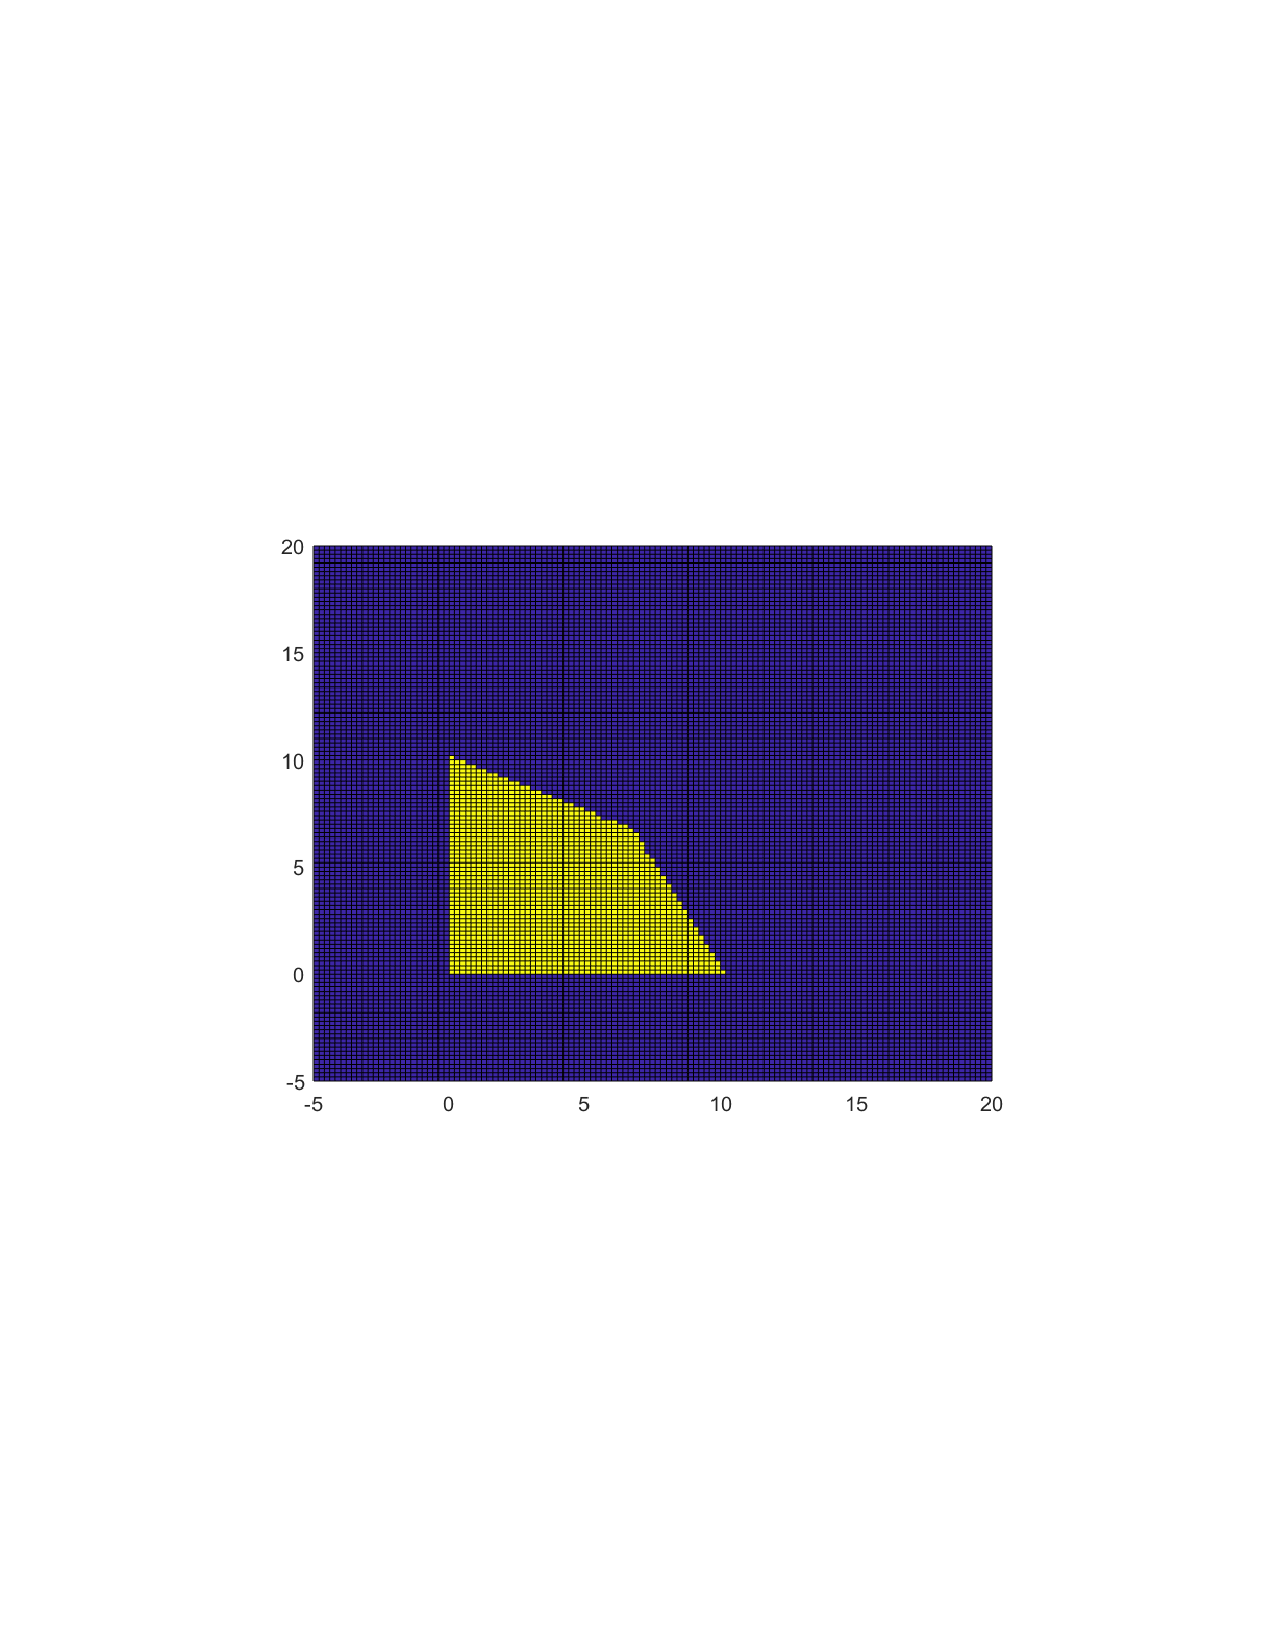
\includegraphics[width=0.3\textwidth]{SimplexFeasibleRegion.pdf} 
\end{center}
\end{figure}

Let's write $x_1$ as the following from the above equalities:
$$
x_1 + 2x_2 \le 20 \implies x_1 \le 20- 2x_2
$$

To calculate where the two inequalities intersect:
\begin{align*}
x_1 + 2x_2 -20 &= 2x_1 + x_2 -20 \\
x_1 + 2x_2 &= 2x_1+x_2 \\
(20-2x_2) + 2x_2 &= 2(20-2x_2) + x_2\\
20 &= 40 - 3x_2 \\
x_2 &= \frac{20}{3} \\
x_1 &= 20 - 2\left(\frac{20}{3}\right) \\
&= \frac{20}{3} \\
(x_1, x_2) &= \left(\frac{20}{3}, \frac{20}{3} \right)
\end{align*}

We check the four corner points of this space to see which point is the minimizer:
\begin{align*}
&(0,0): f(0,0) = -10(0)-12(0) = 0 \\
&(0,10): f(0, 10) = -10(0)-12(10) = -120\\
&(10,0): f(10, 0) = -10(10)-12(0) = -100\\
&(20/3, 20/3): f(20/3, 20/3) = -10(20/3)-12(20/3) = -440/3
\end{align*}

By inspection of the graph we see that the optimal solution is:
$$
(x_1^*, x_2^*) = \left(\frac{20}{3}, \frac{20}{3} \right)
$$

\noindent\textbf{Problem 1.2}

Continuing from in class we now have:
$$
B = \left[\begin{array}{cc} 1 & 1 \\ 2 & 0 \end{array}\right],
B^{-1} = \left[\begin{array}{cc} 0 & 0.5 \\ 1 & -0.5 \end{array}\right],
N = \left[\begin{array}{cc} 2 & 0 \\ 1 & 1 \end{array}\right],
C = \left[\begin{array}{cc} 2 & 0 \\ 1 & 1 \end{array}\right],
c_B = \left[\begin{array}{c} -10 \\ 0 \end{array}\right],
c_N = \left[\begin{array}{c} -12 \\ 0 \end{array}\right]
$$

Update $y$:
\begin{align*}
y &= B^{-1}c_B \\
&= \left[\begin{array}{cc} 0 & 0.5 \\ 1 & -0.5 \end{array}\right]\left[\begin{array}{c} -10 \\ 0 \end{array}\right] \\
&= \left[\begin{array}{c} 0 \\ -10 \end{array}\right]
\end{align*}

Update $z_n$:
\begin{align*}
z_n &= c_N - N^Ty \\
&= \left[\begin{array}{c} -12 \\ 0 \end{array}\right] - \left[\begin{array}{cc} 2 & 1 \\ 0 & 1 \end{array}\right]\left[\begin{array}{c} 0 \\ -10 \end{array}\right] \\
&= \left[\begin{array}{c} -2 \\ 10 \end{array}\right]
\end{align*}

We select $q=2$ as $z_2 = -2 \le 0$:
$$
w = B^{-1}A_2 = \left[\begin{array}{cc} 0 & 0.5 \\ 1 & -0.5 \end{array}\right]\left[\begin{array}{c} 2 \\ 1 \end{array}\right] =
\left[\begin{array}{c} 0.5 \\ 1.5 \end{array}\right]
$$

We set the following:
\begin{align*}
x_2^+ &= \min\left(\frac{(x_B)_1}{w_1}, \frac{(x_B)_2}{w_2}\right) = \min\left(20, \frac{20}{3} \right) = \frac{20}{3} \\
p &= (B)_2 = 3
\end{align*}

We move onto the following updates:
\begin{align*}
x_B^+ &= x_B - wx_q^+ \\
&= \left[\begin{array}{c} 10 \\ 10 \end{array}\right] - \frac{20}{3}\left[\begin{array}{c} 0.5 \\ 1.5 \end{array}\right]\\
&= \left[\begin{array}{c} 20/3 \\ 0 \end{array}\right] \\
x_N &= \left[\begin{array}{c} 20/3 \\ 0 \end{array}\right] \\
x^+ &= \left[\begin{array}{c} 20/3\\ 20/3 \\ 0 \\ 0 \end{array}\right] \\
\mathcal{B}^+ &= \mathcal{B} \cup \{q\} \setminus \{p\} = \{1,3\} \cup \{2\} \setminus \{3\} = \{1,2\}
\end{align*}

And we are finished with the second iteration. Beggining the third:
$$
x = \left[\begin{array}{c}20/3 \\ 20/3 \\ 0 \\ 0 \end{array}\right],
\mathcal{B} = \{1,2\},
\mathcal{N} = \{3,4\},
B = \left[\begin{array}{cc} 1&2 \\ 2&1 \end{array}\right],
N = \left[\begin{array}{cc} 1&0 \\ 0&1 \end{array}\right]
$$
$$
c_N = \left[\begin{array}{c} -12 \\ 0 \end{array}\right],
c_B = \left[\begin{array}{c} -10 \\ -12 \end{array}\right],
c_N = \left[\begin{array}{c} 0 \\ 0 \end{array}\right]
$$

We update $y, z_n$:
\begin{align*}
y &= B^{-1}c_B \\
&= \left[\begin{array}{cc} -1/3 & 2/3 \\ 2/3 & -1/3 \end{array}\right]\left[\begin{array}{c} -10 \\ -12 \end{array}\right]\\
&= \left[\begin{array}{c} -14/3 \\ -8/3 \end{array}\right] \\
z_n &= c_N - N^Ty \\
&= \left[\begin{array}{c} 0 \\ 0 \end{array}\right] - \left[\begin{array}{cc} 1&0 \\ 0&1 \end{array}\right]\left[\begin{array}{c} -14/3 \\ -8/3 \end{array}\right] \\
&= \left[\begin{array}{c} 14/3 \\ 8/3 \end{array}\right]
\end{align*}

And we can terminate the Simplex algorithm as $z_n \ge \vec{0}$. The optimal point is the same found by analysis of the feasible region. 
$$
(x_1^*, x_2^*) = (20/3, 20/3)
$$
\newpage

\section*{Problem 2 {\normalsize [bonus question]}}
In the lecture, we talked about how to choose the initial point for the interior point method by solving two constrained quadratic problems, and we gave solutions for both of them. You are required to give a proof for the second one. More specifically, let $\vA$ be a matrix with full row rank, i.e., $\vA\vA^\top$ is nonsingular. Prove that $\tilde\vy = (\vA\vA^\top)^{-1}\vA\vc$ and $\tilde\vz = \vc-\vA^\top\tilde\vy$ are the solution to the following problem:
$$\argmin_{\vy,\vz} \frac{1}{2}\|\vz\|_2^2, \ \st\ \vA^\top \vy + \vz = \vc.$$

\end{document}
